  \chapter{Wprowadzenie}
  
    Rozwój technologii powoduje zmiany w każdej dziedzinie życia. Dotyka to nie tylko nasze codzienne otoczenie, ale i przede wszystkim gałęzie przemysłu. To właśnie między innymi potrzeby przemysłu napędzają innowacje poprzez wciąż rosnące zapotrzebowanie na nowe, lepsze i wydajniejsze rozwiązania. 
    
    Dzisiejsza technologia pozwala na bardzo precyzyjne sterowanie takim silnikami prądu stałego, a same sterowniki nie zajmują już połowy pokoju. Wręcz przeciwnie - technika analogowa coraz to częściej musi ustępować tej mikroprocesorowej. Powodów takiego stanu rzeczy jest bardzo wiele. Od większej uniwersalności na łatwość poprawy ewentualnych błędów kończąc. 
    
    Jeżeli chodzi jednak o przemysł i produkcję urządzeń na wielką skalę to jest jeden parametr który przyćmiewa wszystkie inne. Są to oczywiście koszty produkcji. Koszty zaprojektowania i wdrożenia produktu na rynek są również ważne, ale to koszty produkcji są powodem dla którego księgowi rwą po nocach włosy z głowy szukając oszczędności na każdym drobnym elemencie. W tym miejscu pojawiają się mikroprocesory. Układy o bardzo dużej wszechstronności, które można w każdej chwili przeprogramować całkowicie zmieniając ich działanie. W rękach sprawnego programisty są bardzo wydajne, a jednocześnie niezwykle energooszczędne. Jednakże w mojej pracy energooszczędność nie jest najważniejszym celem. 
    
    Myślą przewodnią stojącą za powstaniem tego projektu jest zaprojektowanie systemu zdolnego do sterowania pracą silnika prądu stałego. Co więcej, sterowanie odbywać się będzie w sposób zdalny. Jeden sygnał z komputera i sterownik umieszczony nawet na innej półkuli wysteruje silnik tak, jak sobie tego zażyczymy. Projekt dopełniać będzie miła dla oka aplikacja okienkowa, która pozwoli na łatwą obsługę i przejrzysty wgląd w najważniejsze parametry pracy silnika. 
    
    Dodatkowym celem dla projektu jest zachowanie jak najniższej ceny, co będzie później warunkowało wybór konkretnych elementów systemu. Ma to również wpływ na poziom trudności projektu, w szczególności regulatora napięcia elementu wykonawczego, ponieważ tanie elementy cechują znacznie gorsze parametry aniżeli drogie, markowe produkty.
    

 

 

    \section{Zgrubny opis komponentów}
        Projekt opiera się o współpracę trzech kluczowych elementów ciągle komunikujących się ze sobą. Komponenty wchodzące w skład systemu zostały umieszczone na rysunku \ref{fig:system}.
        
        \begin{figure}[ht]
          \centering
          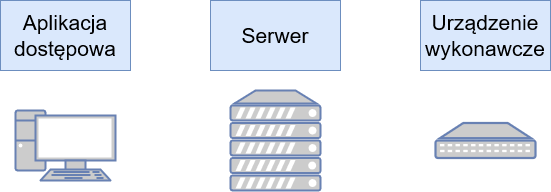
\includegraphics[width=0.9\textwidth]{img/system.png}
          \caption{Elementy systemu}
          \label{fig:system}
        \end{figure}


        \subsection{Aplikacja dostępowa}
            W celu komfortowej obsługi sterownika silnika, została stworzona aplikacja dostępowa w języku C++, która będzie komunikowała się w protokole MQTT. W tym celu wykorzystano otwarto źródłową wersję narzędzia programistycznego jakim jest QT \cite{qt}. Biblioteki QT posiadają dobrze zdefiniowane warstwy abstrakcji oraz bardzo wylewną dokumentację, co sprawia że tworzenie zaawansowanych, przenośnych aplikacji okienkowych jest niezwykle łatwe i przyjemne.
        
        \subsection{Urządzenie wykonawcze}
            Urządzenie końcowe jest dedykowanym rozwiązaniem przygotowanym specjalnie na poczet tego projektu. Bazuje ono na nowoczesnym SoC z rodziny ESP32, który łączy się z brokerem MQTT. Odbierane z niego dane wykorzystane są w procesie sterowania silnikiem. Poza odczytem informacji z brokera, urządzenie publikuje również aktualny stan silnika.
        
        \subsection{Serwer}
            Ostatnim elementem projektu jest Broker MQTT. Jego zadaniem jest bycie łącznikiem pomiędzy urządzeniami. Pozwala on na łatwe subskrybowanie jak i publikowanie informacji. Ta rola przypadła dla otwarto źródłowego brokera Mosquitto wydanego przez fundację Eclipse. Jest to jeden z popularniejszych programów tego typu, a zawdzięcza to małym wymaganiom sprzętowym, skalowalności oraz
            dostępności na wielu architekturach sprzętowych. Co więcej, w celu wdrożenia
            przenośności projektu, oprogramowanie to zostało poddane konteneryzacji,
            dzięki czemu można łatwo transportować go i uruchamiać na innych komputerach wraz z całą konfiguracją przy użyciu ekosystemu Docker.